\documentclass[../report.tex]{subfiles}

\begin{document}

\begin{figure}
\centering
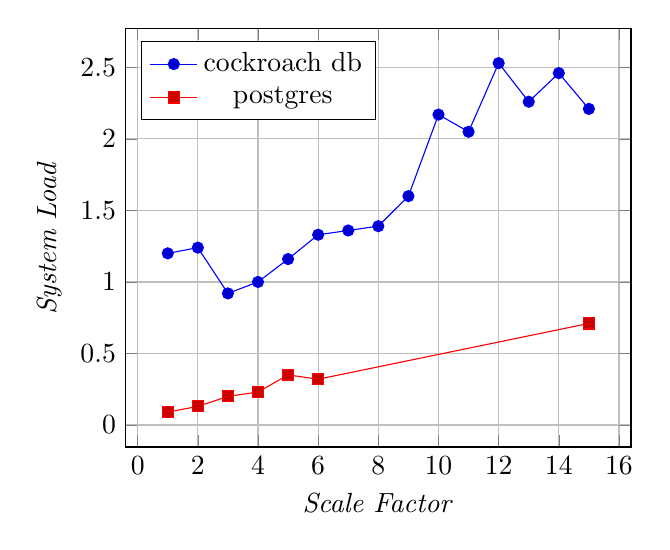
\begin{tikzpicture}[baseline]
    % \begin{axis}[width=7cm, xlabel=\emph{Throughput (req/sec)}, ylabel=\emph{System Load}, ylabel near ticks, grid=major, legend pos=south east, nodes near coords, every node near coord/.append style={font=\footnotesize}, every node near coord/.append style={yshift=-0.5cm}]
    \begin{axis}[width=8cm, xlabel=\emph{Scale Factor}, ylabel=\emph{System Load}, ylabel near ticks, grid=major, legend pos=north west, ytick distance=0.5]
        \addplot coordinates {
            (1,1.2) (2,1.24) (3,0.92) (4,1) (5,1.16) (6,1.33) (7,1.36) (8,1.39) (9,1.60) (10,2.17) (11, 2.05) (12,2.53) (13,2.26) (14,2.46) (15,2.21)
        };
        \addlegendentry{cockroach db}

        \addplot coordinates {
            (1,0.09) (2,0.13) (3,0.2) (4,0.23) (5,0.35) (6,0.32) (15, 0.71)
        };
        \addlegendentry{postgres}
    \end{axis}
\end{tikzpicture}
\label{fig:oltp_load}
\caption{System load during TPC-C benchmark}
\end{figure}

\end{document}
